\section{Experiments}

\problem{experiment\_log}{Experiment logging (3 points)}

For your training and evaluation code, create experiment tracking infrastructure that allows you to track your experiments and loss curves with respect to gradient steps and wallclock time.

\textbf{Deliverable}: Logging infrastructure code for your experiments and an experiment log (a document of all the things you tried) for the assignment problems below in this section.

\begin{answer}
I implemented comprehensive experiment tracking infrastructure using Weights \& Biases (wandb) integrated with Hydra for configuration management. The logging system tracks training and validation losses, learning rates, gradient norms, and wallclock time (recorded by wandb automatically) across all experiments.

All experiment configurations and results are systematically logged and can be accessed through the wandb dashboard for analysis and comparison. A comprehensive code snippet of the logging setup is provided in \ref{appendix:logging-code}. The whole training code is available at \href{https://github.com/donglinkang2021/assignment1-basics/blob/main/train.py}{train.py}. And all the experiment scripts/logs can be found at \href{https://github.com/donglinkang2021/assignment1-basics/tree/main/scripts}{scripts} and \href{https://github.com/donglinkang2021/assignment1-basics/blob/main/docs/CHANGELOG.md}{CHANGELOG.md}.

\end{answer}

\problem{learning\_rate}{Tune the learning rate (3 points) (4 H100 hrs)}

The learning rate is one of the most important hyperparameters to tune. Taking the base model you've trained, answer the following questions:

\begin{enumerate}[label=(\alph*)]
    \item Perform a hyperparameter sweep over the learning rates and report the final losses (or note divergence if the optimizer diverges).
    
    \textbf{Deliverable}: Learning curves associated with multiple learning rates. Explain your hyperparameter search strategy.
    
    \textbf{Deliverable}: A model with validation loss (per-token) on TinyStories of at most 1.45
    
    \item Folk wisdom is that the best learning rate is "at the edge of stability." Investigate how the point at which learning rates diverge is related to your best learning rate.
    
    \textbf{Deliverable}: Learning curves of increasing learning rate which include at least one divergent run and an analysis of how this relates to convergence rates.
\end{enumerate}

\begin{answer}

\textbf{Part (a):}
I employed a logarithmic grid search across learning rates from $10^{-5}$ to $3 \times 10^{-2}$, testing nine values: [1e-5, 3e-5, 1e-4, 3e-4, 1e-3, 3e-3, 6e-3, 1e-2, 3e-2]. Each experiment used identical model architecture and training configuration with cosine learning rate scheduling, 500-step warmup, and AdamW optimizer ($\beta_1=0.9, \beta_2=0.95$, weight decay=0.01). Due to GPU memory constraints (48GB), TinyStories experiments used batch size 256 for 5,000 iterations, while OpenWebText experiments used batch size 128 for 10,000 iterations to maintain total 327,680,000 tokens processed (context length=256). The learning curves are shown in Figure \ref{fig:learning_rate_experiments}.

\begin{figure}[h]
    \centering
    \begin{subfigure}[t]{\textwidth}
        \centering
        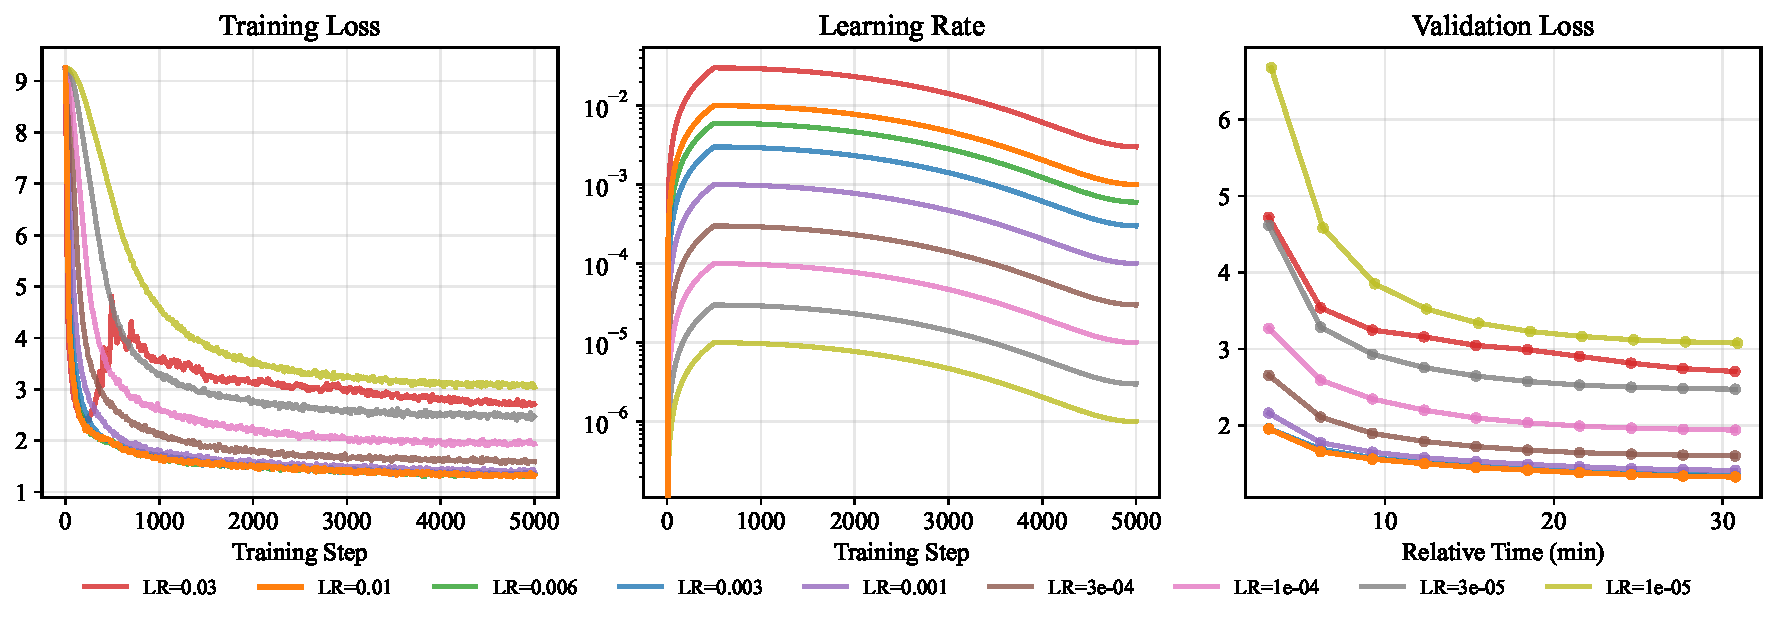
\includegraphics[width=\textwidth]{images/ts_learning_rate_experiments.pdf}
        \vspace{-20pt} % Reduce space between image and caption
        \caption{Learning rate experiments on TinyStories dataset}
        \label{fig:ts_learning_rate_experiments}
    \end{subfigure}
        
    \begin{subfigure}[t]{\textwidth}
        \centering
        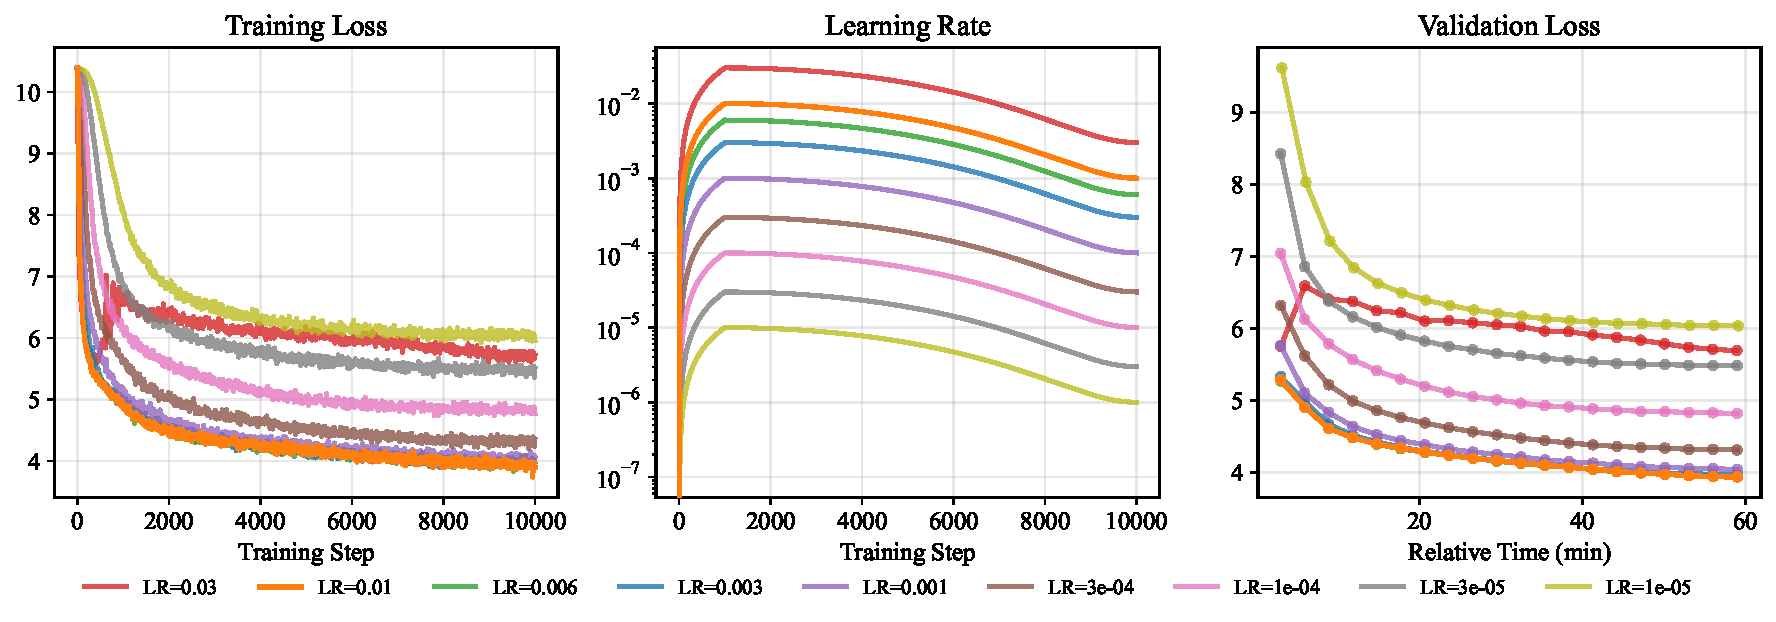
\includegraphics[width=\textwidth]{images/owt_learning_rate_experiments.pdf}
        \vspace{-20pt} % Reduce space between image and caption
        \caption{Learning rate experiments on OpenWebText dataset}
        \label{fig:owt_learning_rate_experiments}
    \end{subfigure}
    
    \caption{Learning rate experiments showing training loss (left), learning rate schedule (middle), and validation loss over time (right) for both datasets. The highlighted orange line represents LR=0.01, which achieved the best performance across both TinyStories and OpenWebText. Complete experiment logs/configs are available on the W\&B: \href{https://api.wandb.ai/links/donglinkang2021-beijing-institute-of-technology/g0usepk4}{Report}.}
    \label{fig:learning_rate_experiments}
\end{figure}

Key findings from both experiments:

- ($\leq 3 \times 10^{-4}$): Stable convergence but inefficient training

- ($1 \times 10^{-3}$ to $1 \times 10^{-2}$): Best balance of convergence speed and stability

- $1 \times 10^{-2}$ achieved val/loss of 1.327, surpassing the target of 1.45 on TinyStories

- $3 \times 10^{-2}$ caused training collapse during warmup at step 480

- OpenWebText experiments mirrored TinyStories results, with $1 \times 10^{-2}$ yielding the best val/loss of 3.93

\textbf{Part (b):}
The "edge of stability" hypothesis suggests optimal learning rates exist just below the divergence threshold. My experiments support this principle:

- $3 \times 10^{-2}$ caused immediate instability during warmup

- $1 \times 10^{-2}$ (approximately 3$\times$ below divergence) achieved the best validation performance

\end{answer}

\problem{batch\_size\_experiment}{Batch size variations (1 point) (2 H100 hrs)}

Vary your batch size all the way from 1 to the GPU memory limit. Try at least a few batch sizes in between, including typical sizes like 64 and 128.

\textbf{Deliverable}: Learning curves for runs with different batch sizes. The learning rates should be optimized again if necessary.

\textbf{Deliverable}: A few sentences discussing of your findings on batch sizes and their impacts on training.

\begin{answer}
I conducted comprehensive batch size experiments on TinyStories, testing values from 1 to 1024: [1, 2, 4, 8, 16, 32, 64, 128, 256, 512, 768, 1024]. All experiments used learning rate $1 \times 10^{-3}$ (selected for better balance of convergence speed and stability), training for 10,000 iterations with the same total token count of 327,680,000 to ensure fair comparison. The learning curves are shown in Figure \ref{fig:batch_size_experiments}.

Key Findings:

- {Small (1-16)}: Exhibited high gradient noise, and increased wall-clock training time despite processing the same number of tokens

- {Optimal (128)}: Achieved the lowest val/loss efficiently (8.75 minutes for 10k iterations)

- {Near (32,64,256,512,768)}: Showed competitive performance, faster per-step computation(256-768)

- {Large (1024)}: Training collapsed, which exceeds memory capacity

\begin{figure}[h]
    \centering
    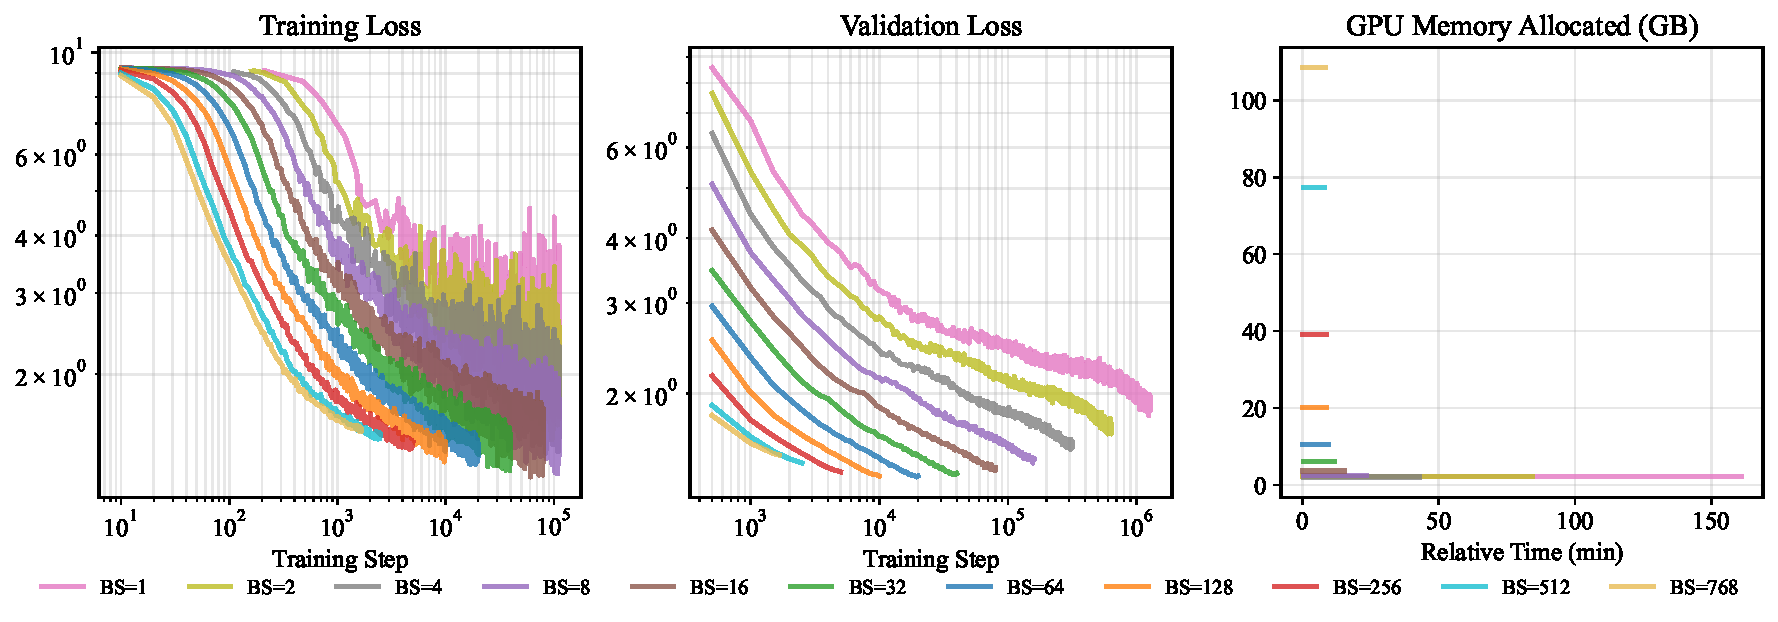
\includegraphics[width=\textwidth]{images/batch_size_experiments.pdf}
    \caption{Batch size experiments on TinyStories showing training loss vs. steps (left, log-log scale), validation loss vs. steps (middle, log-log scale), and GPU memory vs. time (right). Batch size 128 (orange line) achieved the best validation performance with only 8.75 minutes of training time for 10,000 iterations. Complete experiment logs are available on W\&B: \href{https://wandb.ai/donglinkang2021-beijing-institute-of-technology/cs336-assignment1-basics/reports/Batch-size-variations--VmlldzoxNDY5Mzc1OQ?accessToken=5hohvd95f5ejp1e2cn3wt8x2ysqrkgmou352yx2axyiu3ho2fibb3g1bugj39zdx}{Report}.}
    \label{fig:batch_size_experiments}
\end{figure}

\end{answer}

\problem{generate}{Generate text (1 point)}

Using your decoder and your trained checkpoint, report the text generated by your model. You may need to manipulate decoder parameters (temperature, top-$p$, etc.) to get fluent outputs.

\textbf{Deliverable}: Text dump of at least 256 tokens of text (or until the first \lstinline{<|endoftext|>} token), and a brief comment on the fluency of this output and at least two factors which affect how good or bad this output is.

\begin{answer}

Here is a sample of text generated by the best model(val/loss=1.327) from Learning rate experiments on the TinyStories dataset, using max generation length of 1000, a temperature of 0.6 and top-p sampling with p=0.95:

\begin{quote}
Once upon a time, there was a little girl named Lily. She had a doll that she loved very much. The doll was very pretty and expensive. Lily would play with her doll every day and take it with her everywhere she went. One day, Lily and her doll went to the park. They played on the swings and the slide. Lily was having so much fun that she forgot her doll at the park. She forgot about her doll at home. When it was time to go home, Lily's mom called her. Lily was sad because she forgot her doll at the park. She missed her doll and wished she had her doll back. The next day, Lily found her doll at the park and remembered her doll at the park. She ran back to the park and found her doll waiting for her. Lily was so happy to have her doll back and promised to always remember her. Once upon a time, there was a little girl named Sue. She loved to play with her toys and eat yummy food. One day, Sue saw a big, green avocado on the table. She wanted to eat it, but she knew she should ask her mom first. Sue went to her mom and said, "Mom, can I eat the avocado?" Her mom smiled and said, "Yes, you can eat the avocado, but be careful not to break it." Sue was very happy and started to eat the avocado. But then, something unexpected happened. The avocado started to talk! It said, "Please don't eat me!" Sue was very surprised. She did not eat the avocado, but she still loved it very much. Sue and the avocado became best friends. They played and lived happily ever after. Once upon a time, there was a little boy named Tim. He had a big, and he was very tired. He wanted to eat, but he could not. He tried to eat, but he was sad. He had a bad feeling. One day, a lot. She was so close to the day. She was very tired, but she was in the park. She went to the park. She was happy. One day, but a boy was not available. She was not fit in the next to. She went to the day. She felt very well. She was happy. She was a little bit. Once upon a time, there was a little boy, and she had a time. The little girl's house to play. She liked to play area to play. The park. She would go. The little boy's birthdays time to go, but she got a little girl's birthday party. At the park. The park. But, but the park. But, but she could not. She was in the park. She was in the park. The park. Sue's birthday party. Sue's birthday party. Sue's birthday. Sue's birthday to her birthday. At the park. Sue's birthday party. Once there was a big party time, and she had a new season. Sue's birthday, so her mom and her mom's things. Sue's birthdays value her mom's house. Sue, her mom said, her things, and they were not. One day, Sue. She was her house. Sue's birthday. Sue's home. Sue's birthday to go to go to go. Sue's home. Sue's house, but her house. Sue went to go. Sue's room was in a clear that she would be careful not be careful with her mom and she did not to have her mom said, "Mom said, it. Her mom was her mom said, "Please, but also had to remind her mom would not to be careful. She took her mom. She was not. Sue's room for too much better than before she could not. One day, she did not want to eat, "Hi, but not hungry. She said, but not hungry. She wanted her mom, but she would not eat, and she would not. She would open a lot of her mom was always be sad. One day, she was in the whole wide-evia. Avi-evid-so-b at the day. She knew that day. The sun, but the same food was a little boy's mom made a lot of her mom and her mom said thank you, and she thought about the day. Lily and she was a big, and she felt hungry. Lily's day, and her mom said, so much. Lily, but she was a big, and her mom's food to eat, but the day, but the day. Lily's food. The end, and she was not very hungry. Lily was full of a little, and her small, and her favorite food
\end{quote}

\textbf{Comment:}

The generated text shows mixed quality. The first two stories (Lily's doll and Sue's talking avocado) are coherent with proper grammar and logical plots. After ~200 tokens, quality degrades significantly with repetitive phrases ("Sue's birthday party"), incomplete sentences ("He had a big, and he was very tired"), and nonsense ("wide-evia. Avi-evid-so-b").

\textbf{Key factors affecting quality:}

The model uses a 256-token context window during training. Beyond this length, it loses track of earlier content, causing repetition and fragmentation. Maybe the TinyStories dataset contains mostly short stories (<300 tokens), so the model hasn't learned long-form generation. Additionally, with only 22M parameters, the model has limited capacity for complex linguistic patterns and long-range dependencies.

\end{answer}

\problem{layer\_norm\_ablation}{Remove RMSNorm and train (1 point) (1 H100 hr)}

Remove all of the RMSNorms from your Transformer and train. What happens at the previous optimal learning rate? Can you get stability by using a lower learning rate?

\textbf{Deliverable}: A learning curve for when you remove RMSNorms and train, as well as a learning curve for the best learning rate.

\textbf{Deliverable}: A few sentence commentary on the impact of RMSNorm.

\begin{answer}

\end{answer}

\problem{pre\_norm\_ablation}{Implement post-norm and train (1 point) (1 H100 hr)}

Modify your pre-norm Transformer implementation into a post-norm one. Train with the post-norm model and see what happens.

\textbf{Deliverable}: A learning curve for a post-norm transformer, compared to the pre-norm one.

\begin{answer}

\end{answer}

\problem{no\_pos\_emb}{Implement NoPE (1 point) (1 H100 hr)}

Modify your Transformer implementation with RoPE to remove the position embedding information entirely, and see what happens.

\textbf{Deliverable}: A learning curve comparing the performance of RoPE and NoPE.

\begin{answer}

\end{answer}

\problem{swiglu\_ablation}{SwiGLU vs. SiLU (1 point) (1 H100 hr)}

\textbf{Deliverable}: A learning curve comparing the performance of SwiGLU and SiLU feed-forward networks, with approximately matched parameter counts.

\textbf{Deliverable}: A few sentences discussing your findings.

\begin{answer}

\end{answer}

\problem{main\_experiment}{Experiment on OWT (2 points) (3 H100 hrs)}

Train your language model on OpenWebText with the same model architecture and total training iterations as TinyStories. How well does this model do?

\textbf{Deliverable}: A learning curve of your language model on OpenWebText. Describe the difference in losses from TinyStories - how should we interpret these losses?

\textbf{Deliverable}: Generated text from OpenWebText LM, in the same format as the TinyStories outputs. How is the fluency of this text? Why is the output quality worse even though we have the same model and compute budget as TinyStories?

\begin{answer}

\end{answer}

\problem{leaderboard}{Leaderboard (6 points) (10 H100 hrs)}

You will train a model under the leaderboard rules above with the goal of minimizing the validation loss of your language model within 1.5 H100-hour.

\textbf{Deliverable}: The final validation loss that was recorded, an associated learning curve that clearly shows a wallclock-time x-axis that is less than 1.5 hours and a description of what you did. We expect a leaderboard submission to beat at least the naive baseline of a 5.0 loss. Submit to the leaderboard here: \url{https://github.com/stanford-cs336/assignment1-basics-leaderboard}.

\begin{answer}

\end{answer}

